% SPEC-ARCH-07 — Transpositions

% Shared preamble for architecture narrative documents.
% Include from each architecture doc: % Shared preamble for architecture narrative documents.
% Include from each architecture doc: % Shared preamble for architecture narrative documents.
% Include from each architecture doc: \input{./preamble-arch.tex}
% Derived from docs/specs/preamble.tex but tuned for narrative overviews:
% keeps the visual identity, drops contract-specific environments
% (invariant / scenario / ac / Given-When-Then), adds graphicx for
% mermaid-rendered figures.

\documentclass[11pt,a4paper]{article}

\usepackage[utf8]{inputenc}
\usepackage[T1]{fontenc}
\usepackage{lmodern}
\usepackage[a4paper,margin=2.3cm]{geometry}
\usepackage{parskip}
\usepackage{microtype}
\usepackage[dvipsnames]{xcolor}
\usepackage{enumitem}
\usepackage{listings}
\usepackage{titlesec}
\usepackage{fancyhdr}
\usepackage{array}
\usepackage{longtable}
\usepackage{booktabs}
\usepackage{amsmath}
\usepackage{amssymb}
\usepackage{textcomp}
\usepackage{graphicx}
\usepackage{float}
\usepackage{caption}
\usepackage{hyperref}
\usepackage{cleveref}

\definecolor{specBlue}{RGB}{30,64,132}
\definecolor{specGray}{RGB}{90,90,90}
\definecolor{specAccent}{RGB}{198,40,40}
\definecolor{specGreen}{RGB}{30,110,60}

\hypersetup{
  colorlinks=true,
  linkcolor=specBlue,
  urlcolor=specBlue,
  citecolor=specBlue,
  pdfborder={0 0 0}
}

\titleformat{\section}{\Large\bfseries\color{specBlue}}{\thesection}{0.75em}{}
\titleformat{\subsection}{\large\bfseries\color{specBlue!80}}{\thesubsection}{0.6em}{}

\makeatletter
\newcommand{\specID}[1]{\def\@specID{#1}}
\newcommand{\specTitle}[1]{\def\@specTitle{#1}}
\newcommand{\specStatus}[1]{\def\@specStatus{#1}}
\newcommand{\specVersion}[1]{\def\@specVersion{#1}}
\newcommand{\specOwner}[1]{\def\@specOwner{#1}}

\specID{SPEC-ARCH-XX}
\specTitle{Untitled Architecture Doc}
\specStatus{OVERVIEW}
\specVersion{0.1}
\specOwner{Jeremie Nunez}

\newcommand{\makespecheader}{%
  \begin{center}
    {\LARGE\bfseries\color{specBlue}\@specTitle}\\[0.4em]
    {\small\color{specGray}\texttt{\@specID} \quad v\@specVersion \quad \textsc{\@specStatus} \quad \@specOwner}
  \end{center}
  \vspace{0.4em}
  \hrule
  \vspace{0.8em}
}

\pagestyle{fancy}
\fancyhf{}
\fancyhead[L]{\small\color{specGray}\@specID}
\fancyhead[R]{\small\color{specGray}\@specTitle}
\fancyfoot[C]{\small\color{specGray}\thepage}
\renewcommand{\headrulewidth}{0pt}
\makeatother

\captionsetup{font=small,labelfont={bf,color=specBlue},skip=4pt}

\lstdefinestyle{codestyle}{
  basicstyle=\ttfamily\small,
  breaklines=true,
  showstringspaces=false,
  frame=single,
  framesep=4pt,
  rulecolor=\color{specBlue!30},
  backgroundcolor=\color{specBlue!2},
  xleftmargin=0.5em,
  xrightmargin=0.5em,
  keywordstyle=\color{specBlue}\bfseries,
  commentstyle=\color{specGray}\itshape,
  stringstyle=\color{specGreen}
}
\lstset{
  inputencoding=utf8,
  extendedchars=true,
  literate=
    {—}{{--}}1
    {–}{{-}}1
    {…}{{\dots}}1
    {’}{{'}}1
    {‘}{{'}}1
    {“}{{``}}1
    {”}{{''}}1
    {é}{{\'e}}1
    {è}{{\`e}}1
    {ê}{{\^e}}1
    {à}{{\`a}}1
    {â}{{\^a}}1
    {ç}{{\c{c}}}1
    {ô}{{\^o}}1
    {ù}{{\`u}}1
    {→}{{$\to$}}1
    {←}{{$\leftarrow$}}1
    {×}{{$\times$}}1
    {≥}{{$\geq$}}1
    {≤}{{$\leq$}}1
    {≠}{{$\neq$}}1
    {∈}{{$\in$}}1
    {∞}{{$\infty$}}1
    {α}{{$\alpha$}}1
    {β}{{$\beta$}}1
    {μ}{{$\mu$}}1
    {σ}{{$\sigma$}}1
    {·}{{\textperiodcentered}}1
    {⅔}{{2/3}}1
    {⁻}{{\textsuperscript{-}}}1
    {⁴}{{\textsuperscript{4}}}1
}
\lstdefinelanguage{TypeScript}{
  keywords={const,let,var,function,return,if,else,for,while,class,interface,type,extends,implements,import,export,from,as,async,await,new,this,true,false,null,undefined,void,any,unknown,never,string,number,boolean,readonly,private,public,protected,enum},
  sensitive=true,
  comment=[l]{//},
  morecomment=[s]{/*}{*/},
  morestring=[b]",
  morestring=[b]',
  morestring=[b]`
}
\lstset{style=codestyle}

% Derived from docs/specs/preamble.tex but tuned for narrative overviews:
% keeps the visual identity, drops contract-specific environments
% (invariant / scenario / ac / Given-When-Then), adds graphicx for
% mermaid-rendered figures.

\documentclass[11pt,a4paper]{article}

\usepackage[utf8]{inputenc}
\usepackage[T1]{fontenc}
\usepackage{lmodern}
\usepackage[a4paper,margin=2.3cm]{geometry}
\usepackage{parskip}
\usepackage{microtype}
\usepackage[dvipsnames]{xcolor}
\usepackage{enumitem}
\usepackage{listings}
\usepackage{titlesec}
\usepackage{fancyhdr}
\usepackage{array}
\usepackage{longtable}
\usepackage{booktabs}
\usepackage{amsmath}
\usepackage{amssymb}
\usepackage{textcomp}
\usepackage{graphicx}
\usepackage{float}
\usepackage{caption}
\usepackage{hyperref}
\usepackage{cleveref}

\definecolor{specBlue}{RGB}{30,64,132}
\definecolor{specGray}{RGB}{90,90,90}
\definecolor{specAccent}{RGB}{198,40,40}
\definecolor{specGreen}{RGB}{30,110,60}

\hypersetup{
  colorlinks=true,
  linkcolor=specBlue,
  urlcolor=specBlue,
  citecolor=specBlue,
  pdfborder={0 0 0}
}

\titleformat{\section}{\Large\bfseries\color{specBlue}}{\thesection}{0.75em}{}
\titleformat{\subsection}{\large\bfseries\color{specBlue!80}}{\thesubsection}{0.6em}{}

\makeatletter
\newcommand{\specID}[1]{\def\@specID{#1}}
\newcommand{\specTitle}[1]{\def\@specTitle{#1}}
\newcommand{\specStatus}[1]{\def\@specStatus{#1}}
\newcommand{\specVersion}[1]{\def\@specVersion{#1}}
\newcommand{\specOwner}[1]{\def\@specOwner{#1}}

\specID{SPEC-ARCH-XX}
\specTitle{Untitled Architecture Doc}
\specStatus{OVERVIEW}
\specVersion{0.1}
\specOwner{Jeremie Nunez}

\newcommand{\makespecheader}{%
  \begin{center}
    {\LARGE\bfseries\color{specBlue}\@specTitle}\\[0.4em]
    {\small\color{specGray}\texttt{\@specID} \quad v\@specVersion \quad \textsc{\@specStatus} \quad \@specOwner}
  \end{center}
  \vspace{0.4em}
  \hrule
  \vspace{0.8em}
}

\pagestyle{fancy}
\fancyhf{}
\fancyhead[L]{\small\color{specGray}\@specID}
\fancyhead[R]{\small\color{specGray}\@specTitle}
\fancyfoot[C]{\small\color{specGray}\thepage}
\renewcommand{\headrulewidth}{0pt}
\makeatother

\captionsetup{font=small,labelfont={bf,color=specBlue},skip=4pt}

\lstdefinestyle{codestyle}{
  basicstyle=\ttfamily\small,
  breaklines=true,
  showstringspaces=false,
  frame=single,
  framesep=4pt,
  rulecolor=\color{specBlue!30},
  backgroundcolor=\color{specBlue!2},
  xleftmargin=0.5em,
  xrightmargin=0.5em,
  keywordstyle=\color{specBlue}\bfseries,
  commentstyle=\color{specGray}\itshape,
  stringstyle=\color{specGreen}
}
\lstset{
  inputencoding=utf8,
  extendedchars=true,
  literate=
    {—}{{--}}1
    {–}{{-}}1
    {…}{{\dots}}1
    {’}{{'}}1
    {‘}{{'}}1
    {“}{{``}}1
    {”}{{''}}1
    {é}{{\'e}}1
    {è}{{\`e}}1
    {ê}{{\^e}}1
    {à}{{\`a}}1
    {â}{{\^a}}1
    {ç}{{\c{c}}}1
    {ô}{{\^o}}1
    {ù}{{\`u}}1
    {→}{{$\to$}}1
    {←}{{$\leftarrow$}}1
    {×}{{$\times$}}1
    {≥}{{$\geq$}}1
    {≤}{{$\leq$}}1
    {≠}{{$\neq$}}1
    {∈}{{$\in$}}1
    {∞}{{$\infty$}}1
    {α}{{$\alpha$}}1
    {β}{{$\beta$}}1
    {μ}{{$\mu$}}1
    {σ}{{$\sigma$}}1
    {·}{{\textperiodcentered}}1
    {⅔}{{2/3}}1
    {⁻}{{\textsuperscript{-}}}1
    {⁴}{{\textsuperscript{4}}}1
}
\lstdefinelanguage{TypeScript}{
  keywords={const,let,var,function,return,if,else,for,while,class,interface,type,extends,implements,import,export,from,as,async,await,new,this,true,false,null,undefined,void,any,unknown,never,string,number,boolean,readonly,private,public,protected,enum},
  sensitive=true,
  comment=[l]{//},
  morecomment=[s]{/*}{*/},
  morestring=[b]",
  morestring=[b]',
  morestring=[b]`
}
\lstset{style=codestyle}

% Derived from docs/specs/preamble.tex but tuned for narrative overviews:
% keeps the visual identity, drops contract-specific environments
% (invariant / scenario / ac / Given-When-Then), adds graphicx for
% mermaid-rendered figures.

\documentclass[11pt,a4paper]{article}

\usepackage[utf8]{inputenc}
\usepackage[T1]{fontenc}
\usepackage{lmodern}
\usepackage[a4paper,margin=2.3cm]{geometry}
\usepackage{parskip}
\usepackage{microtype}
\usepackage[dvipsnames]{xcolor}
\usepackage{enumitem}
\usepackage{listings}
\usepackage{titlesec}
\usepackage{fancyhdr}
\usepackage{array}
\usepackage{longtable}
\usepackage{booktabs}
\usepackage{amsmath}
\usepackage{amssymb}
\usepackage{textcomp}
\usepackage{graphicx}
\usepackage{float}
\usepackage{caption}
\usepackage{hyperref}
\usepackage{cleveref}

\definecolor{specBlue}{RGB}{30,64,132}
\definecolor{specGray}{RGB}{90,90,90}
\definecolor{specAccent}{RGB}{198,40,40}
\definecolor{specGreen}{RGB}{30,110,60}

\hypersetup{
  colorlinks=true,
  linkcolor=specBlue,
  urlcolor=specBlue,
  citecolor=specBlue,
  pdfborder={0 0 0}
}

\titleformat{\section}{\Large\bfseries\color{specBlue}}{\thesection}{0.75em}{}
\titleformat{\subsection}{\large\bfseries\color{specBlue!80}}{\thesubsection}{0.6em}{}

\makeatletter
\newcommand{\specID}[1]{\def\@specID{#1}}
\newcommand{\specTitle}[1]{\def\@specTitle{#1}}
\newcommand{\specStatus}[1]{\def\@specStatus{#1}}
\newcommand{\specVersion}[1]{\def\@specVersion{#1}}
\newcommand{\specOwner}[1]{\def\@specOwner{#1}}

\specID{SPEC-ARCH-XX}
\specTitle{Untitled Architecture Doc}
\specStatus{OVERVIEW}
\specVersion{0.1}
\specOwner{Jeremie Nunez}

\newcommand{\makespecheader}{%
  \begin{center}
    {\LARGE\bfseries\color{specBlue}\@specTitle}\\[0.4em]
    {\small\color{specGray}\texttt{\@specID} \quad v\@specVersion \quad \textsc{\@specStatus} \quad \@specOwner}
  \end{center}
  \vspace{0.4em}
  \hrule
  \vspace{0.8em}
}

\pagestyle{fancy}
\fancyhf{}
\fancyhead[L]{\small\color{specGray}\@specID}
\fancyhead[R]{\small\color{specGray}\@specTitle}
\fancyfoot[C]{\small\color{specGray}\thepage}
\renewcommand{\headrulewidth}{0pt}
\makeatother

\captionsetup{font=small,labelfont={bf,color=specBlue},skip=4pt}

\lstdefinestyle{codestyle}{
  basicstyle=\ttfamily\small,
  breaklines=true,
  showstringspaces=false,
  frame=single,
  framesep=4pt,
  rulecolor=\color{specBlue!30},
  backgroundcolor=\color{specBlue!2},
  xleftmargin=0.5em,
  xrightmargin=0.5em,
  keywordstyle=\color{specBlue}\bfseries,
  commentstyle=\color{specGray}\itshape,
  stringstyle=\color{specGreen}
}
\lstset{
  inputencoding=utf8,
  extendedchars=true,
  literate=
    {—}{{--}}1
    {–}{{-}}1
    {…}{{\dots}}1
    {’}{{'}}1
    {‘}{{'}}1
    {“}{{``}}1
    {”}{{''}}1
    {é}{{\'e}}1
    {è}{{\`e}}1
    {ê}{{\^e}}1
    {à}{{\`a}}1
    {â}{{\^a}}1
    {ç}{{\c{c}}}1
    {ô}{{\^o}}1
    {ù}{{\`u}}1
    {→}{{$\to$}}1
    {←}{{$\leftarrow$}}1
    {×}{{$\times$}}1
    {≥}{{$\geq$}}1
    {≤}{{$\leq$}}1
    {≠}{{$\neq$}}1
    {∈}{{$\in$}}1
    {∞}{{$\infty$}}1
    {α}{{$\alpha$}}1
    {β}{{$\beta$}}1
    {μ}{{$\mu$}}1
    {σ}{{$\sigma$}}1
    {·}{{\textperiodcentered}}1
    {⅔}{{2/3}}1
    {⁻}{{\textsuperscript{-}}}1
    {⁴}{{\textsuperscript{4}}}1
}
\lstdefinelanguage{TypeScript}{
  keywords={const,let,var,function,return,if,else,for,while,class,interface,type,extends,implements,import,export,from,as,async,await,new,this,true,false,null,undefined,void,any,unknown,never,string,number,boolean,readonly,private,public,protected,enum},
  sensitive=true,
  comment=[l]{//},
  morecomment=[s]{/*}{*/},
  morestring=[b]",
  morestring=[b]',
  morestring=[b]`
}
\lstset{style=codestyle}


\specID{SPEC-ARCH-07}
\specTitle{One-step transposition --- Threat Intelligence and beyond}
\specStatus{OVERVIEW}
\specVersion{0.1}
\specOwner{Jeremie Nunez}

\begin{document}
\makespecheader

\section{Thesis}

Same orchestrator. Same cortex pattern. Same nano swarm. Same HITL sweep. Same guardrails. The transposition is a schema rename + a new fetcher bundle.

\begin{figure}[H]
  \centering
  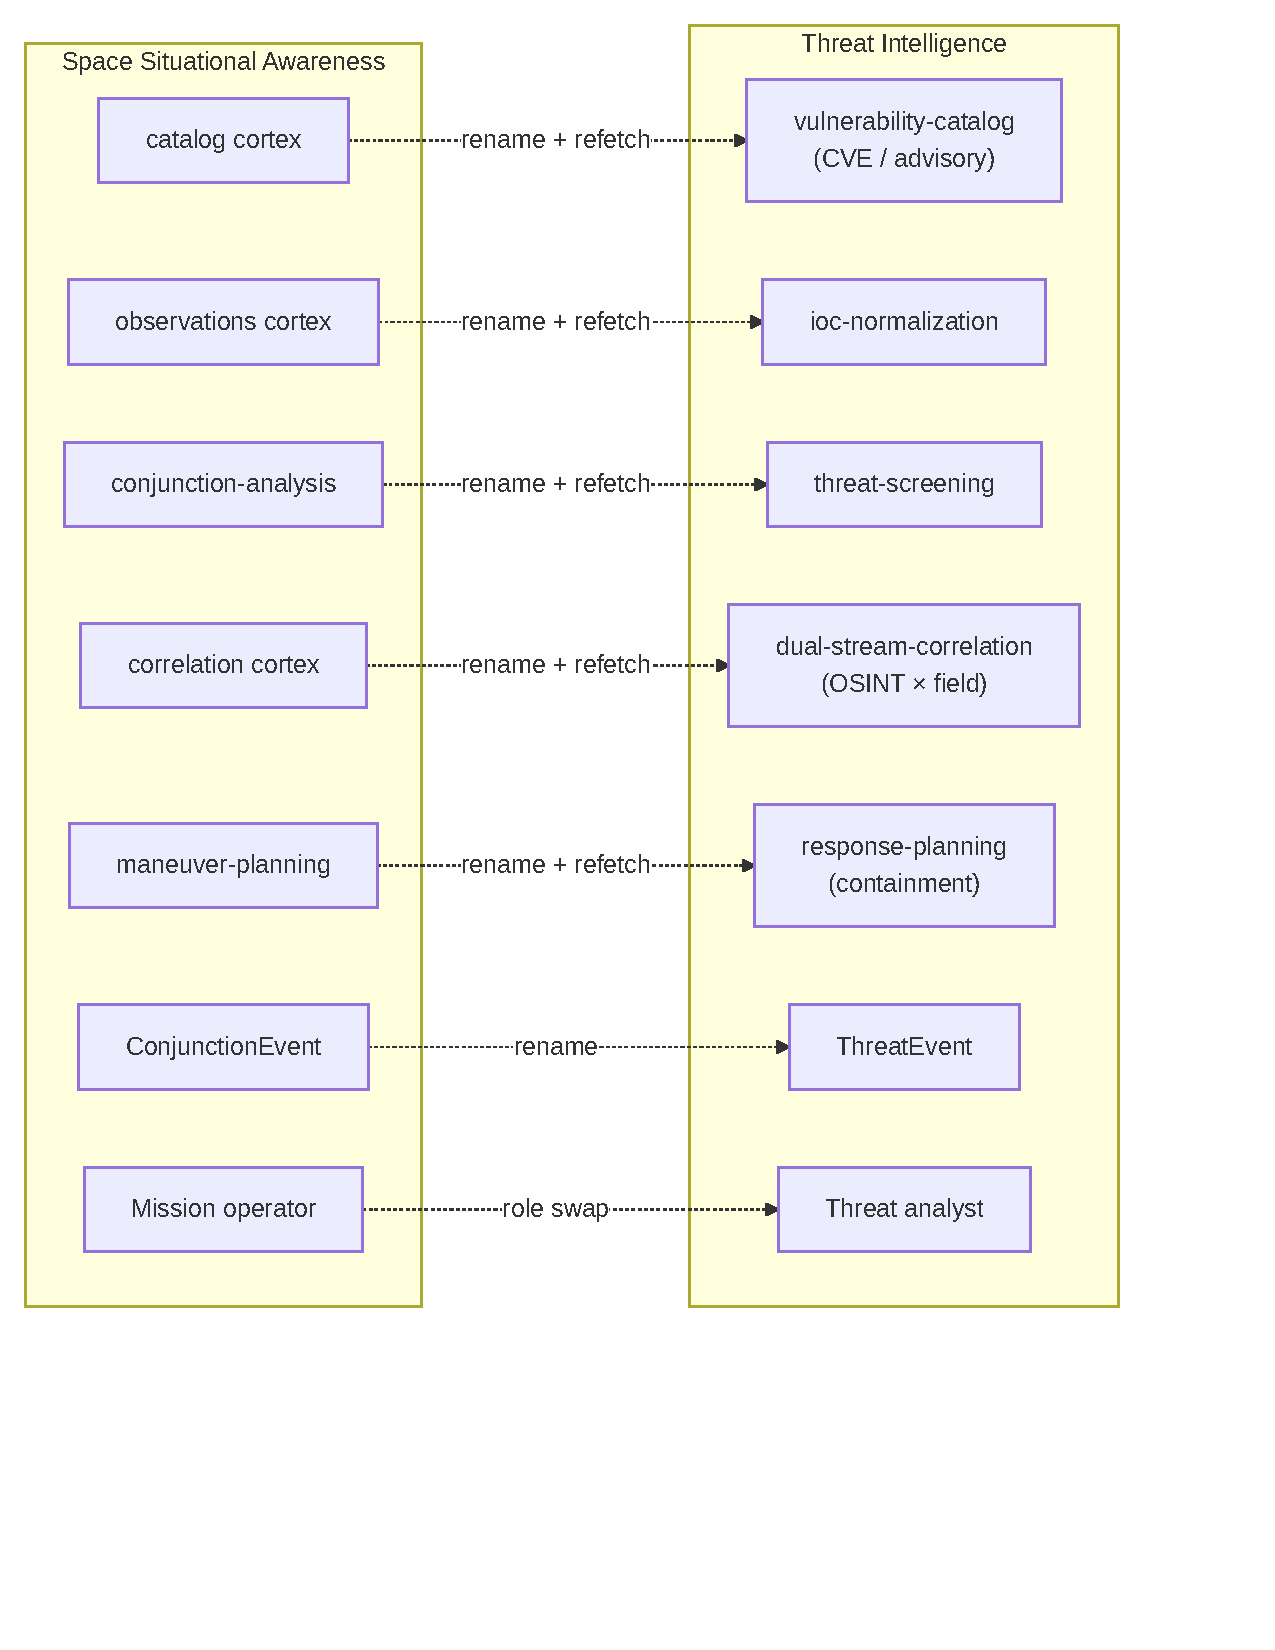
\includegraphics[width=\linewidth]{figures/07-ssa-to-threat-intel.pdf}
  \caption{Cortex-by-cortex mapping from Space Situational Awareness to Threat Intelligence --- every arrow is a rename + refetch, never a rewrite.}
  \label{fig:arch-07-ti}
\end{figure}

\section{What changes per transposition}

\begin{longtable}{@{}lll@{}}
\toprule
\textbf{Layer} & \textbf{Changed} & \textbf{Unchanged} \\
\midrule
\endhead

Schema (entities)   & rename          & --- \\
Skill prompts (.md) & domain-specific & --- \\
Source fetchers     & new bundle      & --- \\
Orchestrator        & ---             & kept \\
Cortex pattern      & ---             & kept \\
Nano swarm          & ---             & kept \\
HITL loop           & ---             & kept \\
Guardrails          & ---             & kept \\
Confidence model    & ---             & kept \\
Audit trail         & ---             & kept \\

\bottomrule
\end{longtable}

\section{Other transpositions (available on request)}

\begin{figure}[H]
  \centering
  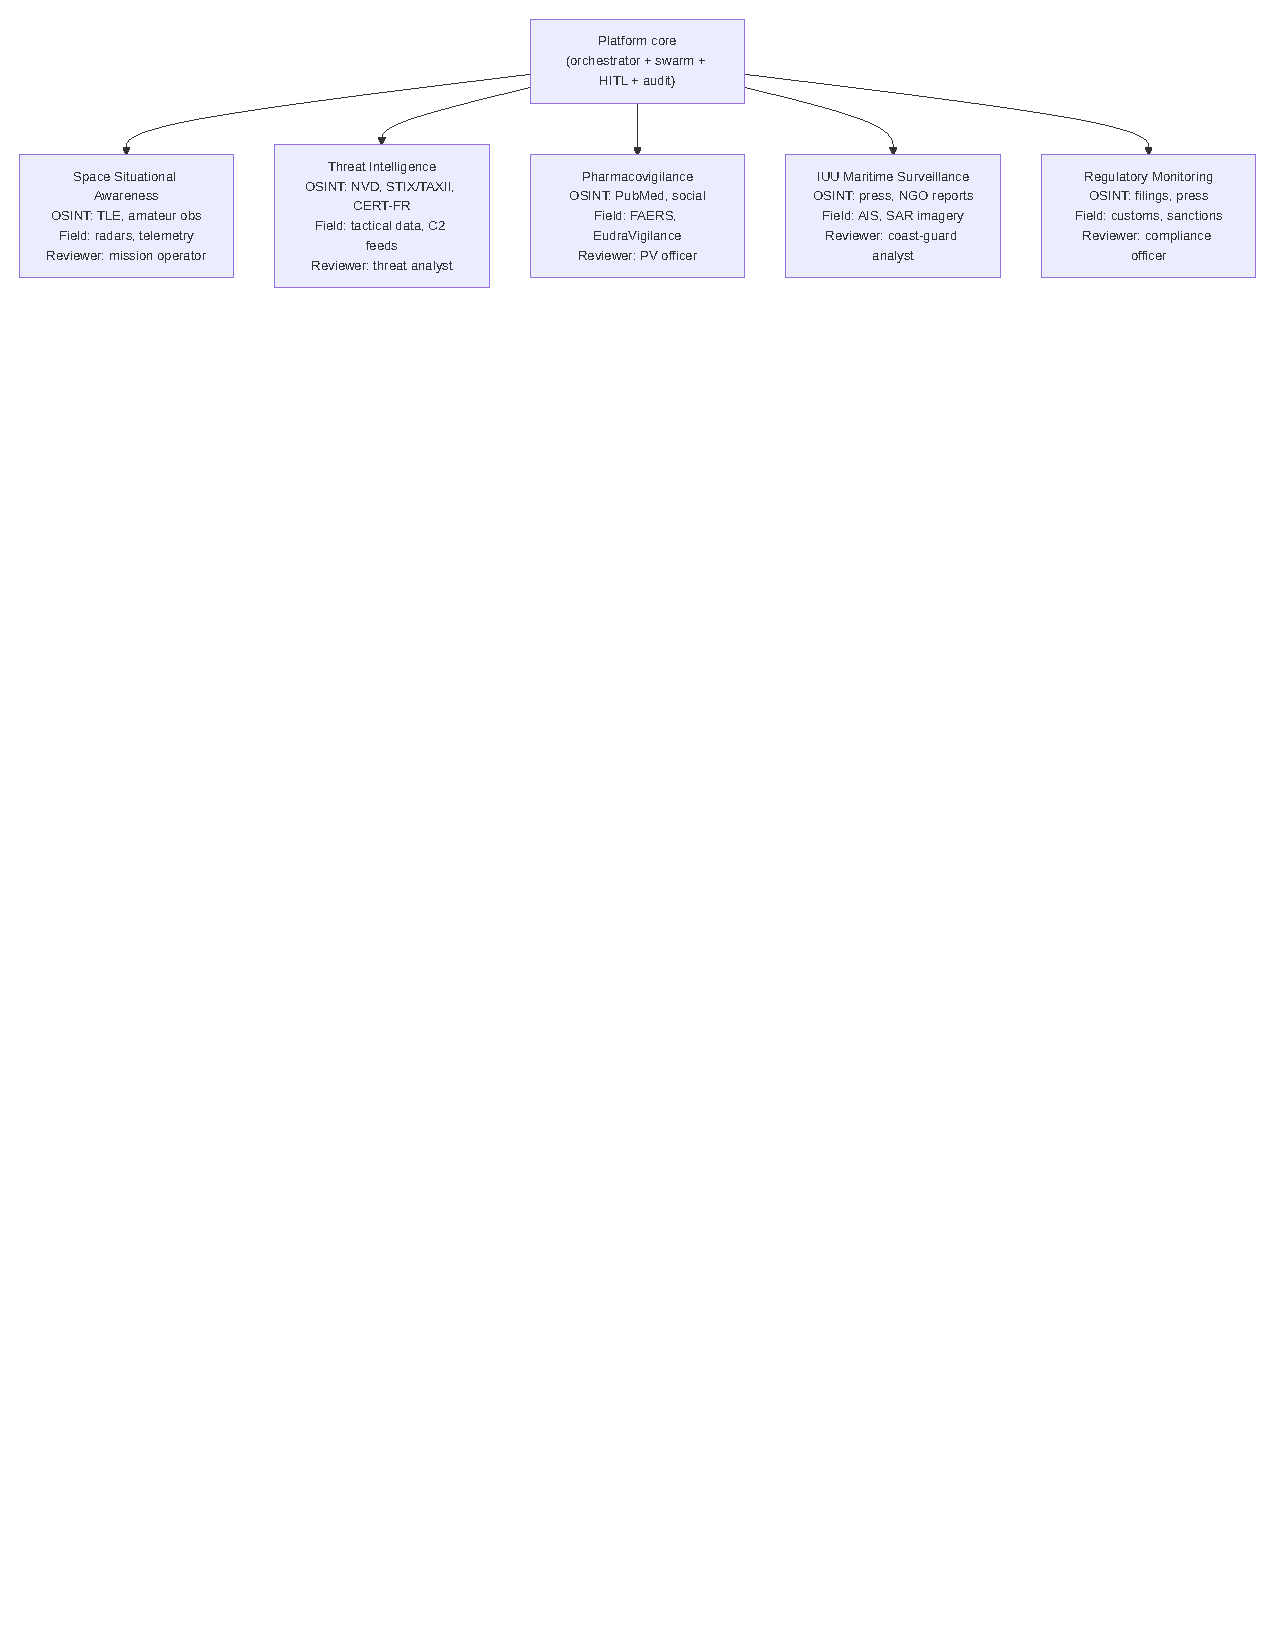
\includegraphics[width=\linewidth]{figures/07-platform-transpositions.pdf}
  \caption{One platform core, five critical-system verticals. Each is a schema + skill-pack swap.}
  \label{fig:arch-07-platform}
\end{figure}

Each uses the same \texttt{docs/specs/} contracts. Each is a schema + skill-pack swap. None requires a new orchestrator, a new swarm, or a new HITL loop.

\section{What each domain actually does}

Same architectural loop --- \emph{OSINT drafts, Field corroborates, human decides, system commits} --- applied to five different critical-system contexts. The substance of each column is what each stream carries, what the cortices compute, and what the reviewer is accountable for.

\begin{longtable}{@{}p{0.11\linewidth}p{0.21\linewidth}p{0.21\linewidth}p{0.22\linewidth}p{0.20\linewidth}@{}}
\toprule
\textbf{Domain} & \textbf{OSINT stream} & \textbf{Field stream} & \textbf{Cortices compute} & \textbf{Reviewer decides} \\
\midrule
\endhead

\textbf{SSA} &
CelesTrak / Space-Track TLEs (days-stale), amateur optical observers, launch-industry press, operator socials &
Classified phased-array radar tracks, operator-owned ephemerides, on-board telemetry &
Orbital propagation (SGP4), close-approach screening with regime-conditioned covariance, Foster-1992 $P_c$ on each pair &
Whether to burn delta-v now, burn later, or keep monitoring --- the \texttt{Maneuver} is audited and reversible from the ledger \\

\textbf{Threat Intelligence} &
NVD / CVE feeds, STIX-TAXII advisories, CERT-FR / ANSSI bulletins, MITRE ATT\&CK updates, vendor blogs, underground chat &
Tactical data-link traces, sensor-fusion bus, C2 telemetry, friendly-force tracking, mission debrief &
Exploitability $\times$ exposure scoring, IoC-to-asset fan-out, lateral-path projection, dwell-time anomaly &
Whether to contain, patch, or observe --- every response action writes an audit row with the analyst's rationale \\

\textbf{Pharmacovigilance} &
PubMed abstracts, ClinicalTrials.gov entries, patient forums, pharmacist social posts, press releases &
FAERS (FDA), EudraVigilance (EMA), VigiBase (WHO), prescriber-EHR signals routed through the sponsor's gateway &
Disproportionality (PRR, ROR), temporal clustering per ATC code, severity-weighted signal detection &
Whether a signal crosses into a regulatory reporting obligation (EMA good practice --- not negotiable, clock starts at receipt) \\

\textbf{IUU maritime} &
Press, NGO reports (Global Fishing Watch, EJF), port-authority bulletins, crew testimony, fleet-owner socials &
AIS transponder tracks, Sentinel-1 SAR dark-vessel detection, coastal radar, VMS from flag-state authorities &
\emph{Dark-vessel detection}: AIS gap $\geq N$ hours overlapping a SAR blob in an EEZ; transshipment pairing by rendezvous pattern; flag-hopping from registry diffs; gear-type inference from speed/heading profile &
Whether to dispatch a coast-guard interdiction, issue a port-state measure, or escalate to a flag-state complaint --- every action auditable for court admissibility \\

\textbf{Regulatory / export} &
Public filings (SEC / AMF), corporate press, procurement postings, trade press &
Customs manifests, dual-use control lists, sanctions registries (OFAC, EU, UN), banking transaction gateways &
Beneficial-owner fan-out, end-user diversion risk, shipping-route plausibility vs.\ declared manifest &
Whether to clear a transaction, block it, or flag for enhanced due diligence --- compliance-officer signature required \\

\bottomrule
\end{longtable}

\end{document}
